\section{Solução desenvolvida}\label{sec:solucao-desenvolvida}

\begin{figure*}[ht]
\centering
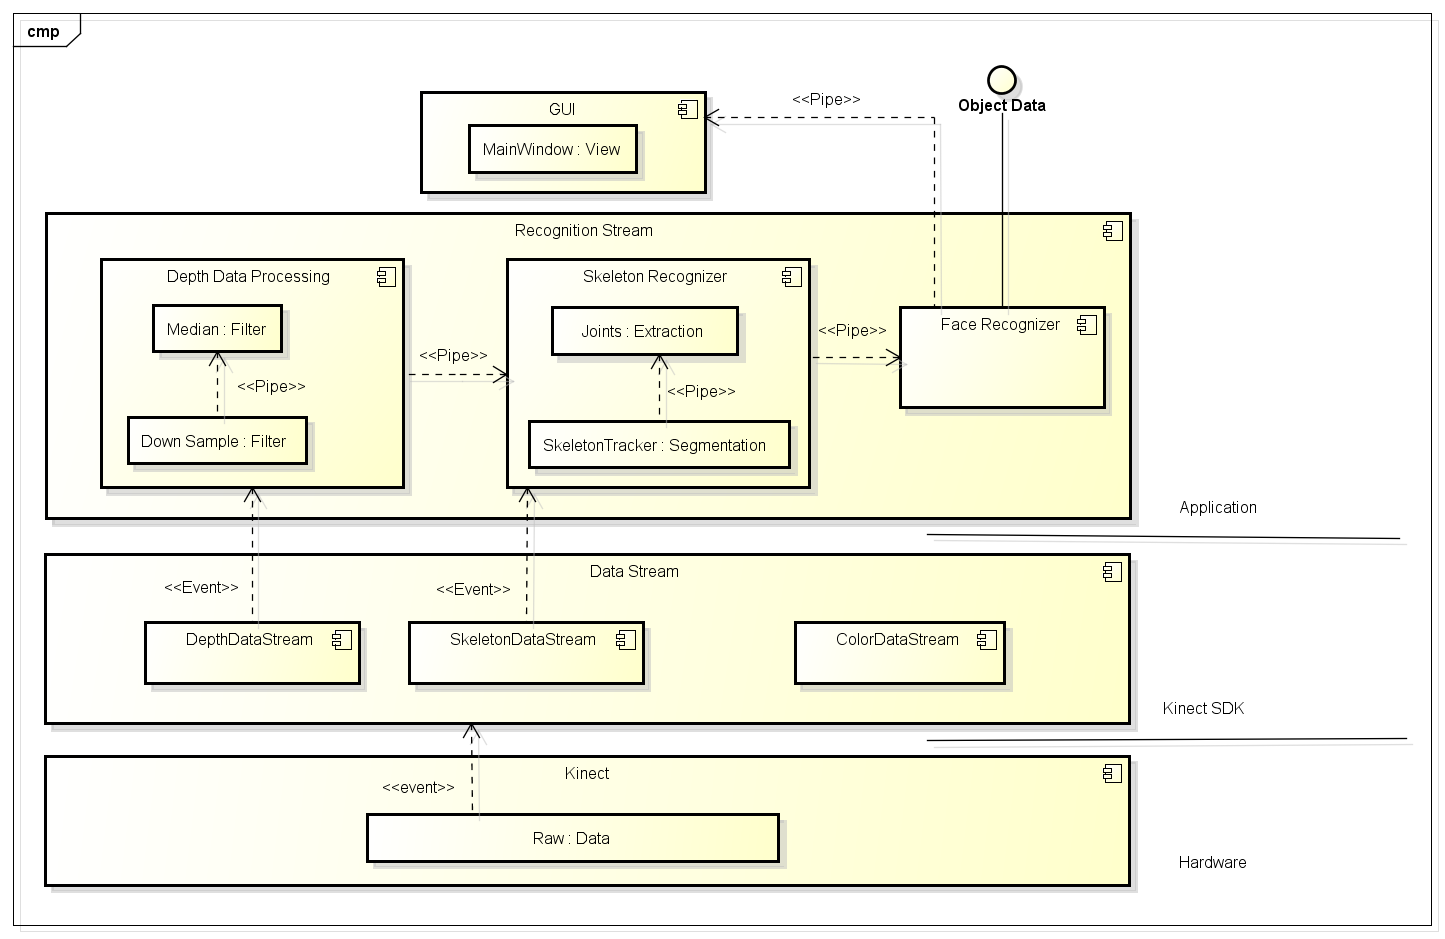
\includegraphics[width=1.0\textwidth]{images/Arquitetura_da_solucao.png}
\caption{Arquitetura da solução proposta}
\label{fig:visao-geral}
\end{figure*}

Motivado pela demanda de serviços de identificação de pessoas e pelo fato de que as soluções para tal problema ainda permanecem em aberto, este trabalho propõe a utilização de mapas de profundidade. O mecanismo de identificação consiste em extrair esse mapa através do projetor infravermelho e do sensor monocromático, e analisar os dados obtidos, utilizando de filtros e algoritmos de segmentação. Por fim, é exibida graficamente uma visualização do mapa de profundidade gerado e, em caso de positivo, o(s) indivíduo(s) encontrado(s) na cena. É exibido também os dados que podem ser exportados para plataformas externas: a localização aproximada dos sujeitos no plano 3D (posições $X$, $Y$ e $Z$) e a distância em relação ao \textit{Kinect}. Nesta seção é discutida a solução desenvolvida.

\subsection{Arquitetura da solução}\label{sec:arqSol}
Para processar os dados de profundidade do sensor \textit{Kinect}, a aplicação executa o seguinte fluxo de dados:

\begin{enumerate}
    \item Habilitar o canal de fluxo de profundidade com o tipo de formato de imagem em profundidade; 
    \item Anexar o manipulador de eventos ao canal de fluxo; 
    \item Processar os quadros de profundidade de entrada; 
    \item Renderizar os quadros na UI.
\end{enumerate}

O \textit{Kinect} é o responsável por obter a visualização da cena de um ambiente interno. Como discutido na seção \ref{sec:trabalhos-relacionados}, o \textit{Kinect} é um sensor de movimento muito eficiente, extraindo com precisão objetos, pessoas e detalhes de uma cena. A \textit{Microsoft} provê para o \textit{Kinect} um Kit de desenvolvimento de software (\textit{Software Development Kit}, SDK). O sistema é composto por módulos adicionados à camada de aplicação, Sobre a camada do SDK. A Figura \ref{fig:visao-geral} apresenta uma visão geral da solução.

\subsubsection{Estilos arquiteturais}\label{sec:estilosArq}
A solução apresenta um estilo arquitetural híbrido, com características de três estilos arquiteturais básicos:

\begin{itemize}
\item Baseado em invocação implícita: \textit{Event Based}; 
\item Baseado em fluxo de dados: \textit{Pipe and Filter}; 
\item Em camadas: \textit{Virtual Machine}.
\end{itemize}

O estilo baseado em eventos (\textit{Event Based}) é um estilo arquitetônico baseado na invocação implícita que fornece uma interação indireta entre componentes acoplados de forma livre, facilitando a adaptação e melhorando a escalabilidade do sistema. Os componentes do tipo de evento (\textit{Depth}, \textit{color} e \textit{Infrared}.) comunicam-se apenas através de eventos transmitidos por um conector de evento.
Este conector então retransmite os eventos para todos os componentes do tipo \textit{Observer} mostrando interesse no evento em questão (Nesse caso, o \textit{Recognition Stream}), melhorando assim a eficiência da distribuição de eventos.

\textit{Pipes} e Filtros (\textit{Pipe and Filter}) é um estilo arquitetural composto por uma cadeia de elementos de processamento, dispostos de forma tal que a saída de cada elemento é a entrada do próximo. O fluxo de dados se dá através de \textit{pipes} (canos) e os dados sofrem transformações quando processados nos filtros. Em outras palavras, os \textit{pipes} é que possibilitam o fluxo dos dados, e os filtros fazem o processamento dos mesmos, colocando-os nos \textit{pipes} antes que todos os dados de entrada sejam consumidos. Portanto, a nível de arquitetura, o processamento é mapeado em filtros e os \textit{pipes} agem como condutores de dados. O componente \textit{Recognition Stream} é composto por subcomponentes do tipo \textit{Filter} e a comunicação entre os mesmos se dá através dos conectores do tipo \textit{Pipe}. 

As arquiteturas de máquinas virtuais (\textit{Virtual Machines}) têm como objetivo alcançar a qualidade da portabilidade. Este estilo de arquitetural simula algumas funcionalidades que não são originais para o \textit{hardware} e/ou \textit{software} em que é implementado. O estilo é aplicado entre o \textit{Kinect (hardware)} e a aplicação desenvolvida, usando conectores do tipo \textit{Event} e \textit{Pipe} entre as camadas. Esse estilo arquitetônico reduz a complexidade, melhora a modularidade, reutilização e manutenção.
Conforme visto na figura \ref{fig:visao-geral}, o sistema possui as camadas:

\begin{itemize}
\item \textit{Kinect (hardware)};
\item \textit{Kinect} SDK; 
\item Aplicação; 
\end{itemize}

\subsubsection{Arquitetura do \textit{Kinect for Windows} SDK}\label{sec:kinectSDK}
O SDK fornece uma biblioteca e ferramentas de software sofisticadas para ajudar os desenvolvedores a usar a forma rica de entrada natural baseada no uso do \textit{Kinect}, que detecta e reage a eventos do mundo real. O \textit{Kinect} e a biblioteca de software interagem com aplicações, como mostrado na Figura \ref{fig:sdk_interact}. Os componentes do SDK são exibidos na figura \ref{fig:sdk_architecture_color} e incluem:

\begin{figure}[h]
\centering
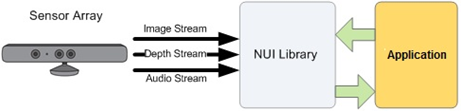
\includegraphics[width=0.5\textwidth]{images/sdk_interaction.png}
\caption{Interação de Hardware e Software com a Aplicação}
\label{fig:sdk_interact}
\end{figure}



\begin{enumerate}
    \item \textit{Hardware Kinect} - Os componentes de \textit{hardware}, incluindo o sensor \textit{Kinect} e o \textit{hub} USB através dos quais o sensor \textit{Kinect} está conectado ao computador;
    \item \textit{Drivers Kinect} - Os \textit{drivers} do Windows para o \textit{Kinect}, que são instalados como parte do processo de configuração do SDK. Os \textit{drivers} do \textit{Kinect} suportam:
        \begin{itemize}
            \item A matriz de microfones como um dispositivo de áudio em modo \textit{kernel} que pode ser acessado  através das API de áudio padrão no Windows; 
            \item Controles de transmissão de áudio e vídeo para transmissão de áudio e vídeo (cor, profundidade e esqueleto);
            \item Funções de enumeração de dispositivos que permitem que um aplicativo use mais de um \textit{Kinect}.	
        \end{itemize} 
    \item Componentes de Áudio e Vídeo:
        \begin{itemize}
            \item Interface de usuário natural do Kinect para rastreamento de esqueleto, áudio e imagem em cores e profundidade. 
        \end{itemize}
    \item Objeto de mídia DirectX (DMO) para formatação de feixes de microfone e localização de fonte de áudio;
    \item API padrão do Windows - APIs de áudio, voz e mídia no Windows, conforme descrito no SDK do Windows e no Microsoft \textit{Speech} SDK.
\end{enumerate}


\subsection{Componentes principais}\label{sec:componentes}

\subsubsection{Color Data Stream}\label{sec:colorDataStream}
O \textit{Kinect} SDK fornece uma classe base abstrata \textit{ImageStream}. Essa classe é implementada tanto pelas classes de \textit{stream} de cores quanto de profundidade. Para a classe \textit{ColorImageStream}, o fluxo é realizado pelos seguintes passos: ativa o fluxo, captura o fluxo quadro a quadro no aplicativo e processsa os quadros de imagens recebidas.

Quando o sensor está em execução, e o fluxo de cores está habilitado, o fluxo irá inicializar o sensor \textit{Kinect} para gerar um fluxo de imagens coloridas. A próxima etapa do fluxo é informar ao sensor o que fazer quando for capturado um novo \textit{frame} de imagem. Para tal, é utilizado um manipulador de eventos que deve ser anexado ao canal do fluxo do sensor. O método \textit{ColorStream.Enable} é um método sobrecarregado que por \textit{default} não recebe argumento, gerando uma resolução de  640x480 \textit{pixels} a 30Fps. Essa resolução default é a utilizada nesse projeto. A classe \textit{KinectSensor} possui um evento \textit{ColorFrameReady}, que é invocado sempre que há novo quadro enviado pelo sensor. O manipulador de eventos possui dois argumentos: o primeiro é um remetente e o segundo um \textit{ColorImageFrameReadyEventArgs}.

\begin{minted}{csharp}
this.sensor = KinectSensor.KinectSensors.
  FirstOrDefault(sensorItem => 
  sensorItem.Status == 
  KinectStatus.Connected);
this.StartSensor();
this.sensor.ColorStream.Enable();
this.sensor.ColorFrameReady += 
  sensor_ColorFrameReady;
\end{minted}


Uma vez que o manipulador de eventos é chamado, significa que há um novo quadro que foi enviado pelo sensor e é hora de processá-lo. Os argumentos do evento para este manipulador de eventos expõem um método \textit{OpenColorImageFrame()} que retorna um \textit{frame} de imagem do tipo \textit{ColorImageFrame}. Com isso, o controle da aplicação se move para o Manipulador de eventos \textit{sensor\_ColorFrameReady} responsável por designar os dados da camera RGB para o devido  processamento do quadro de imagem no \textit{Skeleton Recognizer}. 




\subsubsection{Depth Data Stream}\label{sec:depthDataStream}
\textcolor{red}{capturing data stream}

Quando se trata do Kinect, há apenas uma imagem, que é capturada pelo sensor de profundidade IR. Então, como funciona a triangulação estéreo? Na verdade, existem duas imagens em vez de uma. A segunda imagem é invisível - é um padrão do emissor IR, já definido com o laser IR. O laser IR não é modulado. Tudo o que o laser faz é projetar um padrão pseudo-aleatório de especificações no ambiente Kinect. Essas duas imagens não são equivalentes, pois há alguma distância entre o emissor IR e o sensor de profundidade IR. Essas duas imagens são consideradas como correspondência para diferentes câmeras e permitem a aplicação de triangulação estéreo para calcular a profundidade como mostrado na imagem \ref{fig:trilatStereo}. Essa imagem demonstra como $x1$ e $x2$ são medidos usando a triangulação estéreo para um ponto $X$ na cena. 

\begin{figure}[!h]
\centering
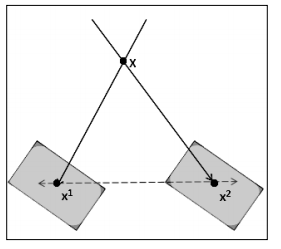
\includegraphics[width=0.4\textwidth]{images/trilateracao_estereo.png}
\caption{Trilateração estéreo para cálculo de profundidade.}
\label{fig:trilatStereo}
\end{figure}

Em um dado pixel $x$, a funcionalidade computa: 


\begin{align}
{f_{\theta}}(I, x) = d_{I}  \left(x + \frac{\boldsymbol{u}}{d_{I}(x)}\right) -  d_{I} \left(x + \frac{\boldsymbol{v}}{d_{I}(x)}\right) ,
\label{eq1}
\end{align}

Onde $d_{I}(x)$ é a profundidade do pixel $x$ na imagem $I$ e os parâmetros $\theta = (\boldsymbol{u,v})$ descreve os \textit{offsets} $\boldsymbol{u}$ e $\boldsymbol{v}$. A normalização dos \textit{offsets} por $\frac{1}{d_{I}(x)}$ garante que os recursos sejam invariantes de profundidade: em um determinado ponto do corpo, um deslocamento de espaço fixo resultará se o pixel está próximo ou longe da câmera. Os recursos são, portanto, invariantes de translação 3D (efeitos de perspectiva de módulo). Se um \textit{pixel} deslocado estiver no fundo ou fora dos limites da imagem, a sonda de profundidade $d_{I}(x')$ recebe um grande valor constante positivo.

o \textit{Depth Data Stream} lê os pontos na cena, processa os dados, de acordo com a equação \ref{eq1} e envia a informação de profundidade a partir da qual eles foram refletidos, para o \textit{Recognition Stream}. Nele, é identificado o sensor \textit{Kinect} conectado e é ativado o canal do fluxo de profundidade.

A classe \textit{ImageStream} possui o método \textit{Enable()} sobrecarregado. Por padrão, o sensor permite o fluxo de profundidade com o formato de imagem de profundidade de resolução 640x480 \textit{pixels} e 30 frames por segundo (\textit{Resolution640x480Fps30}).

Uma vez que o sensor é identificado e o fluxo de profundidade está habilitado, é anexado o manipulador de eventos \textit{DepthFrameReady} a um evento que é gerado cada vez que um novo \textit{frame} de profundidade está disponível:

\begin{minted}{csharp}
this.sensor = KinectSensor.KinectSensors[0];
this.sensor.DepthStream.Enable(
  DepthImageFormat.Resolution640x480Fps30);
sensor.DepthFrameReady +=
  new EventHandler
  <DepthImageFrameReadyEventArgs>
    (sensor_DepthFrameReady);
\end{minted}


\begin{figure*}[ht]
\centering
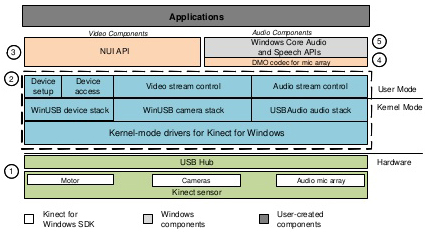
\includegraphics[width=0.8\textwidth]{images/sdk_architecture_color.png}
\caption{Arquitetura do SDK}
\label{fig:sdk_architecture_color}
\end{figure*}


\subsubsection{Depth Data Processing (Recognition Stream - Filter)}\label{sec:depthDataProcessing}
\textcolor{red}{processing data stream}
O manipulador de eventos \textit{DepthFrameReady} invoca com \textit{DepthImageFrameReadyEventArgs}, que possui o método \textit{OpenDepthImageFrame()} para retornar o quadro de imagem de profundidade atual enviado pelo sensor. O  método padrão para \textit{DepthFrameReady} é o \textit{SensorDepthFrameReady}. Nesse método, é recuperado o quadro de imagem em profundidade, usando o método \textit{OpenDepthImageFrame ()}, o qual retorna os dados de profundidade brutos do sensor. \textit{PixelData} cria o tamanho do \textit{buffer} para o quadro de imagem de profundidade de entrada.

O \textit{frame} de profundidade possui propriedades semelhantes que copiam os dados de \textit{pixels} para o \textit{buffer} recém-criado. \textit{CopyPixelDataTo()} é usado para copiar o \textit{array} de bytes de dados de \textit{pixels} do quadro de imagem atualmente recebido para o \textit{buffer}. Antes de copiar os dados de \textit{pixels}, primeiro é calculado o tamanho do \textit{buffer} usando a propriedade \textit{PixelDataLength} e, em seguida, é copiada a mesma imagem do \textit{array} de bytes como \textit{DepthImageFrame}. Como o quadro bruto de imagem de profundidade é uma imagem em escala de cinza de 16 \textit{bits}, \textit{PixelFormats} é especificado  como \textit{Gray16} ao criar a fonte de \textit{bitmap} para o controle de imagem em profundidade.

\textcolor{red}{adicionar aqui os metodos de filtro e segmentação...}


 Na imagem de profundidade gerada pelo \textit{Kinect}, todos os pontos que o sensor não consegue medir a profundidade são deslocados para 0 no \textit{array} de saída. Considerando  como um tipo de ruído, Para evitar sua interferência, é necessário recuperar seu verdadeiro valor de profundidade. Supondo que o espaço seja contínuo, o mais provável é que o ponto faltante tenha um valor de profundidade semelhante aos seus vizinhos. Com esta suposição, todos os 0 \textit{pixels} são considerados como vagos e precisam ser preenchidos. É utilizado então o algoritmo de interpolação vizinho mais próximo para preencher esses \textit{pixels} e obter uma matriz de profundidade que tenha valores significativos em todos os \textit{pixels}. Em seguida, é utilizado o filtro mediano com uma janela 4 x 4 na matriz de profundidade para tornar os dados suaves.

O filtro mediano é uma técnica de filtragem digital não-linear, usada frequentemente para remover o ruído de uma imagem ou sinal. Essa redução de ruído é um passo de pré-processamento típico para melhorar os resultados do processamento posterior (segmentação da uma imagem). A filtragem média é amplamente utilizada no processamento de imagens digitais porque, sob certas condições, preserva bordas ao mesmo tempo que remove o ruído. A idéia principal do filtro mediano é percorrer a entrada do sinal por entrada, substituindo cada entrada pela mediana das entradas vizinhas. O padrão de vizinhos é chamado de "janela", que desliza, entrada por entrada, em todo o sinal. usando um tamanho de janela de três com uma entrada imediatamente anterior e seguindo cada entrada, um filtro mediano é aplicado ao  sinal, como exemplificado, para um conjunto de \textit{pixesls} $x = [2\,80\, 6 \,3]$:

\begin{align*}
x = [2\,\, 80\,\, 6 \,3]\MoveEqLeft[23]\\
y[1] = Mediana[2\,\, 2\,\, 80] = 2\MoveEqLeft[16.7]\\
y[2] = Mediana[2\,\, 80\,\, 6] = Mediana[2\,\, 6\,\, 80] = 6\MoveEqLeft[8]\\
y[3] = Mediana[80\,\, 6\,\, 3] = Mediana[3\,\, 6\,\, 80] = 6\MoveEqLeft[8]\\
y[4] = Mediana[6\,\, 3\,\, 3] = Mediana[3\,\, 3\,\, 6] = 3\MoveEqLeft[9]\\
y = [2\,\, 6\,\, 6\,\, 3]\MoveEqLeft[23].
\end{align*}

Finalmente, é criado o objeto \textit{BitmapSource} e atribuído ao controle de imagem \textit{depthImageControl}, que está definido no arquivo XAML para exibir os dados do fluxo.


\subsubsection{Skeleton recognizer }\label{sec:skeleton}
processing joints

Obter imagem segmentada em profundidade do assunto usando o mapa de profundidade do \textit{Kinect}, já processados pelos filtros. Remover pequenas \textit{blobs}. Obter posições candidatas para a cabeça e a parte superior do corpo utilizando o detector da parte superior do corpo. Corrigir os pontos de cabeça, pescoço e ombro usando os retângulos delimitadores obtidos no passo anterior e dados antropométricos. Calcular a Transformação de Distância Estendida para a imagem de profundidade segmentada. Iniciar uma busca angular para os melhores valores de EDT em torno das articulações do ombro para articulações do cotovelo. Corrige as articulações do cotovelo e levá-las como referência repita o procedimento acima para encontrar a articulação do pulso \textcolor{red}{ver referencia, esta comentada aqui... %(https://people.eecs.berkeley.edu/~akar/IITK_website/cs397/Kinect%20Talk.pdf)
}


O sensor Kinect retorna os dados brutos de profundidade, onde cada pixel contém um valor que representa a distância entre o sensor e o objeto. Os dados de profundidade fornecem possibilidades ilimitadas. Para essa solução, foi necessário obter controle usando o movimento do corpo. Primeiramente é necessário capturar a informação sobre os usuários que estão na frente do Kinect e, a partir desse momento, identificar o mapeamento do esqueleto na imagem.

O recurso completo de rastreamento do esqueleto é construído com base em algoritmos de processamento de dados em profundidade, aprendizado de máquina interna e algoritmos de visão colorida. Usando o rastreamento do esqueleto, o sensor \textit{Kinect} pode rastrear o corpo humano com vários pontos de junção (\textit{joint points}). Usando o \textit{Kinect} é possível detectar até seis indivíduos e até 20 \textit{joints} para cada um deles.



\subsubsection{Face Recognition (Recognition Stream )}\label{sec:depthDataRecognition}
processing data stream


\subsubsection{Main Window (GUI)}\label{sec:mainWindow}
presentating depth map